% =============================================================================
% main.tex — root document for the startup mini-book.
% Build (assignment §13.2):  lualatex -> lualatex -> biber -> lualatex -> lualatex
% or simply: ./build.sh
% =============================================================================
\documentclass[11pt,a4paper,oneside]{report}

% =============================================================================
% preamble.tex — packages, fonts, BiDi, headers/footers, bibliography.
% Engine: LuaLaTeX (assignment §13.2). Compile with: lualatex + biber + lualatex.
% =============================================================================

% --- Page geometry -----------------------------------------------------------
\usepackage[a4paper,margin=2.5cm,headheight=15pt]{geometry}

% --- Fonts + Hebrew/English bidirectional typesetting (babel, bidi=basic) -----
\usepackage{fontspec}
% babel's Unicode bidi engine keeps embedded LTR (English) runs upright inside
% RTL (Hebrew) text and reverses RTL correctly. This is the modern, robust route
% for Hebrew under LuaLaTeX; it replaces polyglossia+luabidi, whose LuaTeX bidi
% mirror-reversed every embedded English run.
\usepackage[bidi=basic]{babel}
\babelprovide[import,main]{hebrew}
\babelprovide[import]{english}

% Hebrew fonts ship with the `culmus` package. This is the ONLY block to change
% for fonts — e.g. swap "David CLM" for "Frank Ruehl CLM" or "Noto Sans Hebrew".
\babelfont{rm}[Script=Hebrew]{David CLM}       % Hebrew serif (main body)
\babelfont{sf}[Script=Hebrew]{Nachlieli CLM}   % Hebrew sans
\babelfont{tt}[Script=Hebrew]{Miriam Mono CLM} % Hebrew monospace
% Latin-script fonts for embedded English / code / math.
\babelfont[english]{rm}{Latin Modern Roman}
\babelfont[english]{tt}{Latin Modern Mono}
\newfontfamily\codefont{Latin Modern Mono}     % inline English code snippets

% --- Colours -----------------------------------------------------------------
\usepackage{xcolor}
\definecolor{brandblue}{HTML}{1F3B73}
\definecolor{brandred}{HTML}{C0392B}
\definecolor{brandgreen}{HTML}{2E7D57}

% --- Graphics, tables, math --------------------------------------------------
\usepackage{graphicx}
% Figures generated by the Python figure service live in ../assets/figures.
\graphicspath{{../assets/figures/}{figures/}}
\usepackage{booktabs}
\usepackage{array}
\usepackage{amsmath}
\usepackage{amssymb}

% --- TikZ (block/flow diagrams, FR-B8) ---------------------------------------
\usepackage{tikz}
\usetikzlibrary{positioning,arrows.meta,shapes.geometric,calc}

% --- Headers / footers (FR-B2) ----------------------------------------------
\usepackage{fancyhdr}
\pagestyle{fancy}
\fancyhf{}
\fancyhead[R]{\small\textbf{כיצד לבנות סטארט-אפ נכון}}
\fancyhead[L]{\small\nouppercase{\leftmark}}
% Force the page number left-to-right: in the Hebrew (RTL) footer, bare two-digit
% numbers could otherwise be reordered by the bidi algorithm (e.g. "14" -> "41").
\fancyfoot[C]{\small\babelsublr{\thepage}}
\renewcommand{\headrulewidth}{0.4pt}
\renewcommand{\footrulewidth}{0.0pt}
\setlength{\headheight}{15pt}

% Chapter-opening pages use the `plain` style. Redefine it so its page number is
% also forced LTR — the default plain footer reversed two-digit numbers under
% babel RTL (the bug that printed "14" as "41" on a chapter's first page).
\fancypagestyle{plain}{%
  \fancyhf{}%
  \fancyfoot[C]{\small\babelsublr{\thepage}}%
  \renewcommand{\headrulewidth}{0pt}%
  \renewcommand{\footrulewidth}{0pt}%
}

% --- Visual design layer (palette, headings, callout/formula boxes) ----------
% =============================================================================
% theme.tex — visual design layer: extended palette, chapter/section styling,
% callout boxes and highlighted formula boxes. Kept separate from preamble so
% each file stays < 150 LOC. Loaded after xcolor + tikz, before hyperref.
% =============================================================================

\usepackage{titlesec}

% --- BiDi-safe TikZ wrapper --------------------------------------------------
% babel bidi=basic reorders node text ACROSS a multi-node picture (only the
% first node keeps its text). Typesetting the whole picture in an LTR (english)
% context fixes it. Node labels must therefore be English — put the Hebrew
% explanation in the figure caption. Usage: \entikz{ \begin{tikzpicture}... }.
\newcommand{\entikz}[1]{\foreignlanguage{english}{#1}}

% --- Extended palette --------------------------------------------------------
\definecolor{ink}{HTML}{1A2433}        % near-black for sub-headings
\definecolor{panel}{HTML}{EEF2F8}      % soft blue tint (callouts)
\definecolor{panelgreen}{HTML}{E9F3EE} % soft green tint (formulas)
\definecolor{rulegrey}{HTML}{C9D3E0}   % light rule under chapter titles

% --- Chapter banner (titlesec) ----------------------------------------------
% A coloured "פרק N" chip, a large brand-blue title, and a thin accent rule.
% NOTE: under babel RTL the ragged directions are mirrored, so \raggedright
% here flushes the chip + title to the RIGHT margin (the Hebrew reading side).
\titleformat{\chapter}[display]
  {\sffamily\bfseries\raggedright}
  {\colorbox{brandblue}{\color{white}\sffamily\bfseries\large\,פרק~\thechapter\,}}
  {0.7ex}
  {\color{brandblue}\Huge\raggedright}
  [\vspace{0.6ex}{\color{rulegrey}\titlerule[1.2pt]}]
\titlespacing*{\chapter}{0pt}{6pt}{1.4ex}

% --- Section / subsection ----------------------------------------------------
\titleformat*{\section}{\sffamily\bfseries\large\color{brandblue}}
\titleformat*{\subsection}{\sffamily\bfseries\color{ink}}

% --- List markers ------------------------------------------------------------
% David CLM has no U+2022 (•), so the default itemize bullet renders as a blank
% "tofu" box. Use a font-independent, on-brand square rule for the first level.
\renewcommand{\labelitemi}{\textcolor{brandblue}{\raisebox{0.25ex}{\rule{0.6ex}{0.6ex}}}}

% --- Coloured callout / formula boxes ----------------------------------------
% Built from \fcolorbox over a captured savebox (NOT tcolorbox, whose frame
% mis-places under babel RTL). The minipage content inherits RTL direction.
% A savebox captures the body first so minipage's internal grouping can't close
% the frame argument early.
\newsavebox{\tkbox}
\newsavebox{\fmbox}

% \begin{takeaway} ... \end{takeaway}  (optional [custom title]).
\newenvironment{takeaway}[1][שורה תחתונה]
  {\par\smallskip\begin{lrbox}{\tkbox}%
   \begin{minipage}{0.90\linewidth}%
   {\sffamily\bfseries\color{brandblue}#1.}\ }
  {\end{minipage}\end{lrbox}%
   \begin{center}\setlength{\fboxsep}{9pt}%
   \fcolorbox{brandblue}{panel}{\usebox{\tkbox}}\end{center}\smallskip}

% \begin{formulabox} \[ ... \] \end{formulabox}
\newenvironment{formulabox}
  {\par\smallskip\begin{lrbox}{\fmbox}%
   \begin{minipage}{0.60\linewidth}\centering}
  {\end{minipage}\end{lrbox}%
   \begin{center}\setlength{\fboxsep}{8pt}%
   \fcolorbox{brandgreen}{panelgreen}{\usebox{\fmbox}}\end{center}\smallskip}


% --- Bibliography (biblatex + biber, FR-B9) ----------------------------------
\usepackage[autostyle=false,style=english]{csquotes}
\usepackage[backend=biber,style=numeric,sorting=none]{biblatex}
\addbibresource{references.bib}

% --- Hyperlinks (linked citations / TOC) -------------------------------------
\usepackage{hyperref}
\hypersetup{
  colorlinks=true,
  linkcolor=brandblue,
  citecolor=brandgreen,
  urlcolor=brandred,
  pdftitle={How to Correctly Build a Start-up},
  pdfauthor={Yosef Shanaa, Ahmad Kais}
}

% --- Convenience macros ------------------------------------------------------
% \en{...} typesets an embedded English (LTR) span inside Hebrew (RTL) text;
% babel keeps it upright and switches to the Latin font + English hyphenation.
\newcommand{\en}[1]{\foreignlanguage{english}{#1}}
% \term{English term} — emphasised inline English term.
\newcommand{\term}[1]{\foreignlanguage{english}{\textit{#1}}}


\begin{document}

% --- Cover (FR-B1) ----------------------------------------------------------
% cover.tex — title / cover page (FR-B1): topic, author, date, course, lecturer.
\begin{titlepage}
\centering
\thispagestyle{empty}

\vspace*{1.2cm}
{\Huge\bfseries כיצד לבנות סטארט-אפ נכון\par}
\vspace{0.4cm}
{\Large מדריך מתומצת: מרעיון לחברה\par}
\vspace{0.3cm}
{\large\en{\itshape How to Correctly Build a Start-up}\par}

\vspace{1.0cm}
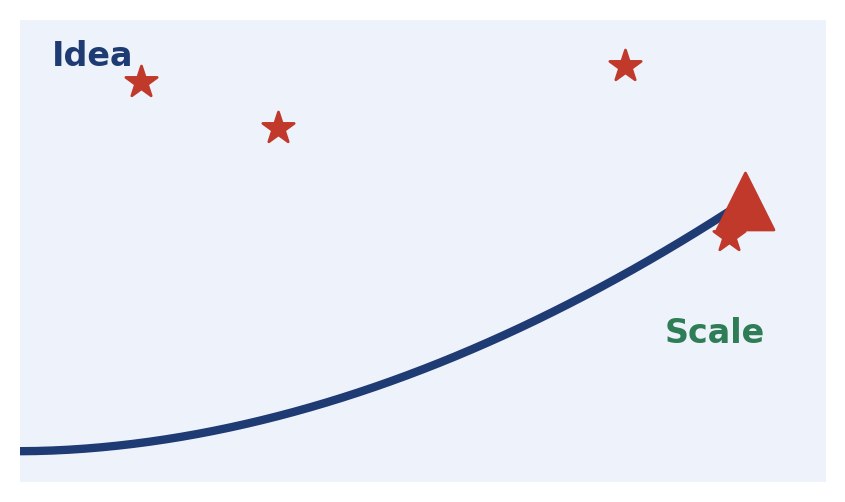
\includegraphics[width=0.66\textwidth]{illustration.png}\par

\vspace{1.0cm}
\begin{tabular}{r@{\hskip 1em}l}
  \textbf{מחבר:}  & \en{yosefshanaa} \\[4pt]
  \textbf{קורס:}  & ייצור המוני של סוכני בינה מלאכותית \\[4pt]
  \textbf{מרצה:}  & ד״ר יורם סגל \\[4pt]
  \textbf{תאריך:} & \today \\
\end{tabular}

\vfill
{\small נוצר באמצעות צוות סוכני \en{CrewAI} והופק ב־\en{LuaLaTeX}.\par}
\end{titlepage}


% --- Table of contents (FR-B2) ----------------------------------------------
\tableofcontents
\thispagestyle{empty}
\clearpage

% --- Chapters ---------------------------------------------------------------
\chapter{מבוא: מהו סטארט-אפ ולמה רובם נכשלים}

\term{startup} אינו סתם עסק קטן. זהו ארגון זמני שנועד לחפש מודל עסקי
\en{(business model)} בר-חזרה והדיר, בתנאי אי-ודאות קיצונית~\cite{blank2013startup}.
ההבדל מהותי: בעל מסעדה מפעיל מודל ידוע, בעוד שיזם סטארט-אפ \emph{מחפש} מודל
שעדיין אינו קיים. מסיבה זו, סטארט-אפ הוא קודם כול \emph{ניסוי} — ולא תוכנית
ביצוע.

הסטטיסטיקה איננה מחמיאה: כשלושה מכל ארבעה סטארט-אפים מגובי הון אינם מחזירים
את ההשקעה, והסיבה השכיחה ביותר לכישלון אינה טכנולוגיה כושלת אלא היעדר ביקוש
אמיתי בשוק~\cite{cbinsights2021}. כלומר, רוב הצוותים בונים מוצר נכון מבחינה
הנדסית — לבעיה הלא-נכונה.

\section{מסע המזומנים של הסטארט-אפ}

הדרך מרעיון לחברה רווחית עוברת כמעט תמיד דרך ``עקומת ה-\en{J}'': תזרים המזומנים
המצטבר צולל תחילה אל מתחת לאפס (שלב השריפה, \term{burn}), מגיע לשפל, ורק לאחר
שההכנסות עוקפות את העלויות הקבועות הוא מטפס חזרה אל הרווחיות. איור~\ref{fig:jcurve}
ממחיש זאת.

\begin{figure}[h]
  \centering
  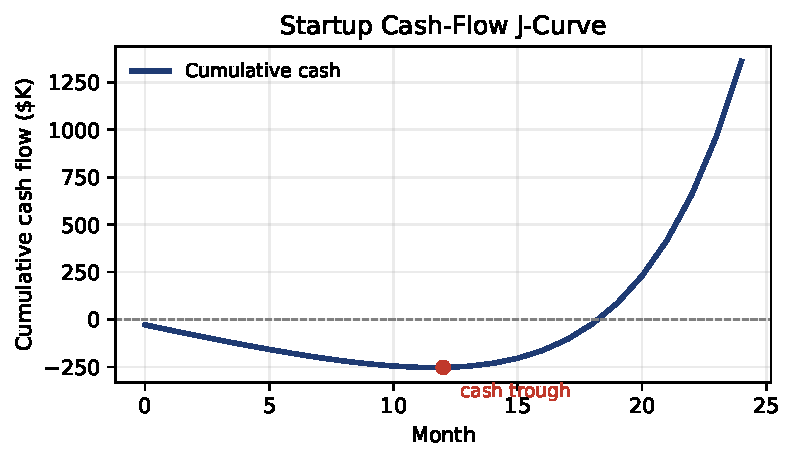
\includegraphics[width=0.78\textwidth]{jcurve.pdf}
  \caption{עקומת ה-\en{J} של תזרים המזומנים המצטבר לאורך 24 חודשים. נקודת השפל
  מסמנת את הרגע שבו דרוש הון נוסף כדי לשרוד עד להתאוששות.}
  \label{fig:jcurve}
\end{figure}

\section{תזת הספר}

ספר זה טוען טענה אחת מרכזית: בניית סטארט-אפ נכון היא \emph{תהליך למידה ממושמע},
לא הימור חד-פעמי. נציג שיטה מסודרת — מאימות הבעיה, דרך לולאת
\term{Build--Measure--Learn}, התאמת מוצר-שוק, בניית הצוות וכלכלת היחידה, ועד
ניהול הסיכונים והטעויות הנפוצות. כל פרק מסתמך על עקרונות שהוכחו בספרות
המקצועית~\cite{ries2011lean,thiel2014zero}.

\chapter{אימות הרעיון ומציאת בעיה אמיתית}

הטעות הנפוצה ביותר בתחילת הדרך היא להתאהב בפתרון במקום בבעיה. רעיונות טובים
לסטארט-אפ נובעים בדרך כלל מבעיה אמיתית שהיזם חווה בעצמו, ולא ממאמץ מכוון
``להמציא רעיון''~\cite{graham2005ideas}. בעיה שכדאי לפתור היא כזו שהיא
\emph{תכופה}, \emph{כואבת} ושהקהל מוכן לשלם כדי להיפטר ממנה.

\section{גילוי לקוחות לפני כתיבת קוד}

מתודולוגיית פיתוח הלקוחות \term{(Customer Development)} גורסת שיש לצאת מחוץ
לבניין ולדבר עם לקוחות פוטנציאליים \emph{לפני} שבונים מוצר~\cite{blank2013startup}.
מטרת השיחות אינה למכור, אלא ללמוד: מהי הבעיה, כיצד הלקוח פותר אותה היום, וכמה
היא עולה לו. שאלות טובות עוסקות בעבר ובהווה (``מתי נתקלת בבעיה לאחרונה?'') ולא
בעתיד ההיפותטי (``האם היית קונה?'').

\section{ניסוח השערות בדיקות}

רעיון הוא אוסף של השערות \term{(hypotheses)} שטרם נבדקו: מי הלקוח, מהי הבעיה,
מה הפתרון, ומדוע ישלמו עליו. עבודה נכונה ממירה כל השערה לניסוי זול ומהיר. אם
ההשערה החשובה ביותר — שקיים ביקוש — אינה מתאמתת, עדיף לגלות זאת תוך שבוע ובעלות
זניחה, ולא לאחר שנה של פיתוח. זהו לב ההיגיון הרזה: \emph{להקטין בזבוז} על ידי
למידה מהירה.

\chapter{שיטת ה-\texorpdfstring{\en{Lean Startup}}{Lean Startup} ולולאת \texorpdfstring{\en{Build--Measure--Learn}}{Build-Measure-Learn}}

\emph{פרק זה מדגים מעבר דו-כיווני} \term{(BiDi)} \emph{נכון בין עברית מימין-לשמאל
לבין מונחי אנגלית וקוד משמאל-לימין.}

שיטת ה-\en{Lean Startup} של אריק ריס מציעה מנוע צמיחה המבוסס על
\emph{למידה מאומתת} \term{(validated learning)}: כל מחזור פיתוח מתחיל בהשערה,
ממיר אותה למוצר מינימלי בר-קיימא — \term{Minimum Viable Product (MVP)} —
ומודד את תגובת הלקוחות בפועל~\cite{ries2011lean}.

\section{לולאת \texorpdfstring{\en{Build--Measure--Learn}}{Build-Measure-Learn}}

ליבת השיטה היא לולאת משוב מהירה: \en{Ideas} $\rightarrow$ \en{Build}
$\rightarrow$ \en{Product} $\rightarrow$ \en{Measure} $\rightarrow$ \en{Data}
$\rightarrow$ \en{Learn}, וחוזר חלילה. המטרה אינה לעבור את הלולאה פעם אחת, אלא
\emph{למזער את הזמן} למחזור שלם. איור~\ref{fig:bml} מתאר את הלולאה.

\begin{figure}[h]
  \centering
  \begin{tikzpicture}[every node/.style={font=\small\itshape}]
    \node[draw, circle, minimum size=1.5cm, fill=brandblue!10] (build) at (0,0) {\en{Build}};
    \node[draw, circle, minimum size=1.5cm, fill=brandgreen!10] (measure) at (3.4,-2.2) {\en{Measure}};
    \node[draw, circle, minimum size=1.5cm, fill=brandred!10] (learn) at (-3.4,-2.2) {\en{Learn}};
    \draw[-{Stealth[length=3mm]}, very thick, brandblue]
      (build) to[bend left=20] node[right=2pt]{\en{Product}} (measure);
    \draw[-{Stealth[length=3mm]}, very thick, brandgreen]
      (measure) to[bend left=20] node[below=2pt]{\en{Data}} (learn);
    \draw[-{Stealth[length=3mm]}, very thick, brandred]
      (learn) to[bend left=20] node[left=2pt]{\en{Ideas}} (build);
  \end{tikzpicture}
  \caption{לולאת \en{Build--Measure--Learn} — מנוע הלמידה של ה-\en{Lean Startup},
  משורטטת ב-\en{TikZ}.}
  \label{fig:bml}
\end{figure}

\section{\texorpdfstring{\en{MVP}}{MVP}, פיבוט ומדדים שאינם משקרים}

ה-\en{MVP} הוא הגרסה הזולה ביותר שעדיין מאפשרת לבדוק את ההשערה המרכזית — לא
מוצר חצי-אפוי, אלא \emph{ניסוי ממוקד}. כאשר הנתונים מלמדים שההשערה שגויה, מבצעים
\emph{פיבוט} \term{(pivot)} — שינוי מבני בכיוון תוך שמירה על מה שנלמד. חשוב להבחין
בין \term{actionable metrics} (מדדים מובילים לפעולה) לבין \term{vanity metrics}
(מדדי יוהרה) כגון מספר הורדות מצטבר, שנראים טוב אך אינם מנחים החלטה.

לדוגמה, השערה נבדקת מנוסחת באנגלית כשורה אחת:
\begin{quote}\en{\codefont If we add one-click checkout, weekly repeat purchases rise by 15\%.}\end{quote}
לאחר ההגדרה הזו חוזרים לעברית: רק כאשר המספר מאומת בנתוני אמת, מקדמים את הפיצ׳ר
משלב הניסוי אל המוצר.
      % BiDi chapter (FR-B7)
\chapter{לקוחות מוקדמים והתאמת מוצר-שוק}

התאמת מוצר-שוק — \term{Product--Market Fit (PMF)} — היא הרגע שבו המוצר פותר בעיה
אמיתית עבור שוק מוגדר, באופן שהשוק ``מושך'' את המוצר מידי הצוות. מארק אנדריסן
תיאר זאת כתחושה שאי אפשר לטעות בה: השרתים קורסים, המכירות רצות מהר מהגיוס,
והצוות בקושי מספיק לתמוך בלקוחות~\cite{andreessen2007pmf}.

\section{מאמצים מוקדמים ולקוחות ראשונים}

לפני \en{PMF}, היעד אינו צמיחה אלא \emph{למידה}. לקוחות מוקדמים
\term{(early adopters)} מוכנים לסבול מוצר לא מושלם משום שהכאב שלהם חריף; הם
מקור המשוב היקר ביותר. בשלב זה עדיף ``לעשות דברים שאינם ניתנים להרחבה'':
לגייס לקוחות ידנית, לתמוך בהם אישית, וללמוד מכל שיחה.

\section{מדידת ההתאמה}

כיצד יודעים שהגענו? סימנים כמותיים כוללים שיעור שימור גבוה
\term{(retention)} שמתייצב ואינו דועך לאפס, ושיעור גבוה של משתמשים המצהירים
שהיו ``מאוכזבים מאוד'' אם המוצר ייעלם. כל עוד אין \en{PMF}, השקעה בשיווק נרחב
היא בזבוז: היא שופכת מים לדלי מחורר. רק לאחר שההתאמה מושגת, עוברים לשלב הצמיחה
ולכלכלת היחידה הנדונה בפרק~\ref{chap:economics}.

\chapter{בניית הצוות המייסד}

המשאב הקריטי ביותר בשלב המוקדם אינו ההון אלא הצוות. פיטר תיל מדגיש שראיון
המפתח אינו ``מדוע הרעיון טוב'', אלא ``מדוע דווקא הצוות הזה'' — האם המייסדים
מכירים זה את זה היטב, משלימים זה את זה, ומחויבים לטווח ארוך~\cite{thiel2014zero}.

\section{תפקידים משלימים}

צוות מייסד בריא משלב יכולות בנייה (\en{building}) ויכולות הפצה (\en{distribution}).
חברה רבת-עוצמה מבחינה טכנולוגית אך חסרת ערוץ הפצה תיכשל לא פחות מחברה עם שיווק
מצוין ומוצר חלש. חלוקת התפקידים צריכה להיות ברורה, אך גבולות הגזרה גמישים דיים
כדי לאפשר עבודה משותפת בתנאי אי-ודאות.

\section{הון אנושי, מניות והסכמות מוקדמות}

חלוקת המניות בין המייסדים והגדרת תקופת הבשלה \term{(vesting)} הן החלטות שכדאי
לקבל מוקדם ובכתב, בעוד היחסים טובים. הסכמות לא-פורמליות הן מקור נפוץ לסכסוכים
מאוחרים שעלולים לפרק את החברה. עיקרון מנחה: לתגמל מחויבות עתידית ולא רק תרומה
היסטורית, וליישר את התמריצים של כל המייסדים עם הצלחת החברה לטווח ארוך.

\section{תרבות וגיוסי העובדים הראשונים}

לאחר המייסדים, עשרת העובדים הראשונים מעצבים את \emph{התרבות} של החברה לשנים
הבאות. בשלב זה כל גיוס הוא החלטה אסטרטגית: עובד לא-מתאים פוגע בצוות קטן הרבה
יותר מאשר בארגון גדול. עדיף לגייס לאט, להעדיף יכולת למידה ותחושת בעלות
\term{(ownership)} על פני ניסיון צר, ולחפש אנשים המתפקדים היטב באי-ודאות.
תרבות אינה סיסמאות על הקיר אלא סך ההתנהגויות שהמייסדים מתגמלים ומענישים בפועל;
היא נקבעת מוקדם, וקשה מאוד לשנותה מאוחר.

\section{קצב, מיקוד ומשמעת ביצוע}

בשלב המוקדם היתרון התחרותי הגדול ביותר של סטארט-אפ הוא \emph{קצב} — היכולת
ללמוד ולשחרר מהר יותר מהמתחרים. קצב נשמר באמצעות מיקוד אכזרי: לבחור בכל רגע
את המשימה האחת החשובה ביותר, ולסרב לעשרות הזדמנויות סבירות שמפזרות את הצוות.
פגישות שבועיות קצרות סביב מדד-על אחד, יחד עם הגדרת ``הצעד הבא הקטן ביותר''
שניתן לשחרר, ממירות חזון מעורפל לתנועה מדידה קדימה.

\chapter{כלכלת יחידה וגיוס הון}
\label{chap:economics}

סטארט-אפ שורד כל עוד יש לו מזומן. כלכלת היחידה \term{(unit economics)} בודקת אם
\emph{לקוח בודד} מרוויח לחברה יותר ממה שעלה לגייסו. שני הגדלים המרכזיים הם
הערך לכל החיים של הלקוח, \en{LTV}, ועלות הרכישה, \en{CAC}.

\section{הנוסחאות המרכזיות}

הערך לכל החיים מוגדר כיחס בין הרווח הגולמי החודשי הממוצע ללקוח לבין שיעור
הנטישה החודשי:
\begin{formulabox}
\[ \mathrm{LTV} \;=\; \frac{\overline{\mathrm{ARPA}} \cdot m_{\text{gross}}}{c_{\text{churn}}} \]
\end{formulabox}
כאשר $\overline{\mathrm{ARPA}}$ הוא ההכנסה הממוצעת לחשבון, $m_{\text{gross}}$
הוא שיעור הרווח הגולמי ו-$c_{\text{churn}}$ הוא שיעור הנטישה החודשי. עלות
הרכישה ומסלול המזומן \term{(runway)} נתונים על ידי:
\begin{formulabox}
\[ \mathrm{CAC} \;=\; \frac{S_{\text{S\&M}}}{N_{\text{new}}}
   \qquad\qquad
   \mathrm{Runway} \;=\; \frac{C_{\text{cash}}}{B_{\text{net}}} \]
\end{formulabox}
כאשר $S_{\text{S\&M}}$ היא הוצאת המכירות והשיווק, $N_{\text{new}}$ מספר הלקוחות
החדשים, $C_{\text{cash}}$ יתרת המזומן ו-$B_{\text{net}}$ קצב השריפה החודשי
נטו. כלל האצבע המקובל לבריאות עסקית הוא:
\begin{formulabox}
\[ \dfrac{\mathrm{LTV}}{\mathrm{CAC}} \;\geq\; 3 \qquad\text{and}\qquad
   \mathrm{CAC\ Payback} \;\leq\; 12\ \text{months} \]
\end{formulabox}

איור~\ref{fig:unit} משווה \en{LTV} מול \en{CAC} בשלושה ערוצי רכישה; היחס מופיע
מעל כל זוג עמודות.

\begin{takeaway}
לפני שמזרימים תקציב לשיווק, ודאו שיחס \en{LTV}/\en{CAC} בריא. גיוס הון מגדיל
את \emph{קנה-המידה} של כלכלת היחידה — אם היחידה מפסידה, ההון רק מאיץ את ההפסד.
\end{takeaway}

\begin{figure}[htbp]
  \centering
  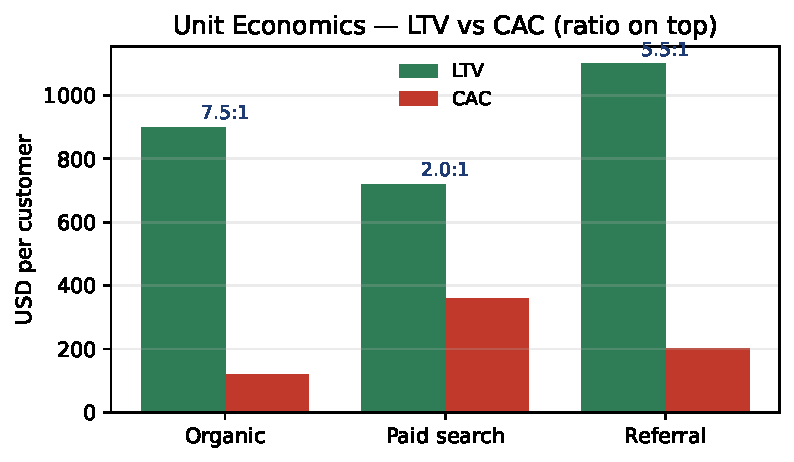
\includegraphics[width=0.78\textwidth]{unit_economics.pdf}
  \caption{כלכלת יחידה — \en{LTV} מול \en{CAC} לפי ערוץ רכישה (גרף שנוצר בקוד
  \en{Python}). ערוץ ה-\en{Referral} מציג את היחס הבריא ביותר.}
  \label{fig:unit}
\end{figure}

\section{שלבי גיוס ההון}

גיוס הון אינו מטרה אלא דלק. כל סבב מתאים לשלב סיכון שונה, ומחירו — דילול
ההחזקה. טבלה~\ref{tab:rounds} מסכמת את השלבים האופייניים.

\begin{table}[htbp]
  \centering
  \caption{שלבי גיוס אופייניים ומיקודם.}
  \label{tab:rounds}
  \begin{tabular}{l r r l}
    \toprule
    \textbf{\en{Stage}} & \textbf{גיוס (\en{\$})} & \textbf{שווי (\en{\$M})} & \textbf{מיקוד עיקרי} \\
    \midrule
    \en{Pre-Seed} & \en{50K--500K}  & \en{1--5}    & אימות בעיה ורעיון \\
    \en{Seed}     & \en{0.5--3M}    & \en{5--20}   & חיפוש התאמת מוצר-שוק \\
    \en{Series A} & \en{3--15M}     & \en{20--80}  & מנוע צמיחה חוזר \\
    \en{Series B} & \en{15--50M}    & \en{80--250} & הרחבה ושוקים חדשים \\
    \bottomrule
  \end{tabular}
\end{table}
 % math formula (FR-B6) + table (FR-B5) + graph (FR-B4)
\chapter{טעויות נפוצות וניהול סיכונים}

ניתוח של מאות כשלונות מצביע על דפוסים חוזרים. הסיבה המובילה לכישלון היא
היעדר צורך אמיתי בשוק, ואחריה אזילת המזומן וצוות לא מתאים~\cite{cbinsights2021}.
איור~\ref{fig:funnel} מציג את שרשרת הסיכונים העיקרית.

\begin{figure}[h]
  \centering
  % English labels + explicit coordinates inside an LTR (\entikz) context, so
  % babel bidi keeps the labels in their boxes. Hebrew meaning is in the caption.
  \entikz{%
  \begin{tikzpicture}[
      box/.style={draw=brandred, rounded corners, minimum width=2.6cm, minimum height=1.1cm,
                  align=center, font=\small, fill=brandred!8},
      arr/.style={-{Stealth[length=3mm]}, very thick, brandred}]
    \node[box] (need) at (0,0)   {No market\\need};
    \node[box] (cash) at (3.3,0) {Ran out\\of cash};
    \node[box] (team) at (6.6,0) {Wrong\\team};
    \node[box] (comp) at (9.9,0) {Out-\\competed};
    \draw[arr] (need) -- (cash);
    \draw[arr] (cash) -- (team);
    \draw[arr] (team) -- (comp);
  \end{tikzpicture}}
  \caption{שרשרת הסיכונים השכיחה לכישלון סטארט-אפ — היעדר צורך בשוק, אזילת מזומן,
  צוות לא מתאים ותבוסה בתחרות (לפי \en{CB Insights}; שורטט ב-\en{TikZ}).}
  \label{fig:funnel}
\end{figure}

\section{אנטי-דפוסים שכדאי להכיר}

\begin{itemize}
  \item \textbf{בנייה מוקדמת מדי:} כתיבת קוד לפני אימות הביקוש — בזבוז המשאב
        היקר ביותר, זמן.
  \item \textbf{הרחבה מוקדמת \term{(premature scaling)}:} השקעה בשיווק וגיוס
        לפני שהושגה התאמת מוצר-שוק.
  \item \textbf{מדדי יוהרה:} מעקב אחר מספרים מרשימים שאינם מנחים החלטה.
  \item \textbf{התעלמות מ-\en{runway}:} אי-ניהול קצב השריפה עד שמתגלה מאוחר
        מדי שאין מספיק מזומן לסבב הבא.
\end{itemize}

\section{ניהול סיכונים כתהליך מתמשך}

ניהול סיכונים אינו אירוע חד-פעמי אלא בקרה שוטפת: לזהות את ההשערה המסוכנת ביותר
בכל רגע, לבדוק אותה בזול, ולעדכן את התוכנית בהתאם. זוהי בדיוק לולאת הלמידה
מפרק~\ref{fig:bml}, מיושמת על קיום החברה עצמה.

\chapter{סיכום ומפת דרכים}

בניית סטארט-אפ נכון אינה הימור על רעיון בודד אלא תהליך למידה ממושמע תחת
אי-ודאות. ראינו כי רוב הכשלונות נובעים מבעיה לא-אמיתית, ולכן הסדר הנכון הוא
\emph{בעיה לפני פתרון}, \emph{למידה לפני הרחבה}, ו\emph{מזומן לפני יוקרה}.

\section{מפת דרכים תמציתית}

\begin{enumerate}
  \item \textbf{בעיה:} זהה בעיה תכופה וכואבת; אמת אותה בשיחות עם לקוחות אמיתיים.
  \item \textbf{\en{MVP}:} בנה ניסוי מינימלי שבודק את ההשערה המסוכנת ביותר.
  \item \textbf{לולאה:} הפעל \en{Build--Measure--Learn} ומזער את זמן המחזור.
  \item \textbf{\en{PMF}:} חתור להתאמת מוצר-שוק לפני כל השקעה בצמיחה.
  \item \textbf{צוות:} בנה צוות מייסד משלים עם הסכמות ברורות מראש.
  \item \textbf{כלכלה:} ודא ש-$\mathrm{LTV}/\mathrm{CAC} \geq 3$ ונהל את ה-\en{runway}.
  \item \textbf{סיכונים:} בדוק בכל רגע את ההשערה המסוכנת ביותר, בזול ובמהירות.
\end{enumerate}

\section{מילה אחרונה}

הכלים שהוצגו — מתודולוגיית הלקוחות, הלולאה הרזה, כלכלת היחידה וניהול הסיכונים —
אינם נוסחת קסם, אלא מסגרת משמעת. הם מגדילים את הסיכוי שהמשאב היקר ביותר, זמנו
של הצוות, יושקע בבעיה הנכונה. זה, בתמצית, ההבדל בין סטארט-אפ שבונה את המוצר
\emph{נכון} לבין סטארט-אפ שבונה את המוצר \emph{הנכון}.


% --- Bibliography (FR-B9) ---------------------------------------------------
\printbibliography[heading=bibintoc]

\end{document}
